\section{Introduction}

% dialogue summarization task
Dialogue summarization is a specialized summarization task that takes
a series of utterances from multiple speakers in the first person as input,
and outputs fluent and concise summaries in third persons as shown in 
\figref{fig:example}. It helps people be acquainted with the gist of a dialogue 
when they jump into a conversation, or review
the key points after a conversation.
Different from previous monologue inputs such as news~\cite{narayan2018don} and scientific publications~\cite{cohan2018discourse}, dialogues are always less well-organized. They usually contain complicated reference relations, inconsecutive inter-utterance dependencies, informal expressions, and so on, making dialogue summarization a more challenging task.

%Compared with previous text summarization tasks which
%mostly focus on news~\cite{narayan2018don} and scientific 
%publications~\cite{cohan2018discourse}, dialogue summarization has
%a few additional challenges: i) the input dialogue is a mix of multiple
%persons' viewpoints, making it difficult to track the co-reference and hence
%\textit{who does what}; ii) dialogues are less organized, and 
%may contain ambiguous or inconsistent inter-utterance dependences; 
%and iii) if the dialogue is oral, the language used maybe less 
%formal and comes with errors and redundancies. 

\begin{figure}
	\centering
	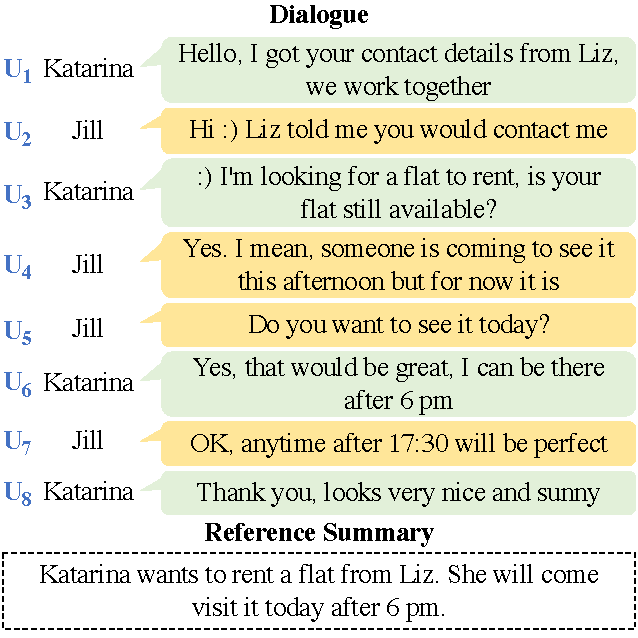
\includegraphics[width=0.85\columnwidth]{example.pdf}
	\caption{An example from SAMSum dataset. Different colors are used 
to identify different speakers.}
	\label{fig:example}
\end{figure}

% pretrain models
The most obvious characteristic of this task is the difference in the format and language styles 
between dialogue and its narrative summary.
Liu, Shi and Chen~\shortcite{liu2021coreference} mentioned
that coreference resolution models trained on general narrative text 
underperforms by about 10\% on dialogue corpus, 
demonstrating the inherent gap between dialogue and narrative text. 
As a result, popular PLMs such as BART~\cite{lewis2020bart} and 
PEGASUS~\cite{zhang2020pegasus} which excel on news summarization 
perform moderately on dialogue summarization.
Therefore, models trained on a single text format, e.g., narrative text, 
are sub-optimal for cross-format tasks, including dialogue summarization.

% makes models trained on narrative text sub-optimal for dialogue-related tasks. 
% previous work
To narrow this gap, previous work on dialogue summarization mainly 
resort to injecting dialogue features into PLMs to enhance dialogue 
understanding. These features include dialogue acts~\cite{goo2018abstractive}, topic transitions~\cite{chen2020multi}, coreference relations~\cite{liu2021coreference}, discourse graphs~\cite{chen2021structure}, etc. 
However, they suffer from two weaknesses. 
First, oracle labeled features are hard to collect and 
errors can propagate from wrong labels to poor summaries.
Most features are annotated by labeling models trained on other corpora. 
Carefully designed rules or hyper-parameters are needed for transferring 
these models to different dialogue summarization datasets, which is 
time-consuming and labor-intensive.
Second, additional layers or more encoders are required to incorporate 
features into PLMs, increasing the GPU memory footprint both during 
training and test.

%First, data labeling approaches are transferred from their original designed domains and need human labors to design different hyper-parameters or rules for adapting to different dialogue summarization datasets, such as the
%weights between two views in Multi-view~\cite{chen2020multi} and 
%rules in~\citet{liu2021coreference}.
%Second, features may not generalize well to different dialogue scenarios. For example, the argument graph~\cite{fabbri2021convosumm} for capturing key argumentative contents is not suitable for e-mail threads as mentioned in their paper. 

% our approach
In this paper, we propose an alternative approach to bridge the gap by post-training PLMs on learning to rephrase from dialogue to narrative text. 
After that, the post-trained model is further fine-tuned as usual 
for dialogue summarization. 
Since there is no dialogue-to-text rephrasing task or related datasets as far as we know, we consider two ways for enhancing the rephrasing ability based on the existing dialogue summarization data.
One way is that we construct paraphrasing datasets with the same amount of information between inputs and outputs and post-train the model with vanilla generation task.
The other way is to design rephrasing learning objectives for utilizing information unbalanced data. We newly introduce the prefix-guided generation (PGG) task, using the first several tokens in the output as supervision. 
Then, the model can learn to rephrase the designated information by prefix into third-person narratives.
%Then, training the model to learn sentence completion in the third-person point of view for rephrasing ability.

%We designed different operations to 
%construct paraphrasing dataset extracted from the existing dialogue-to-summary pairs. 
%One option is to fix the input dialogue and manipulate the utterances into 
%indirect speech by simple rules as the output. Another option is to 
%fix the output, in the form of either a summary or a sentence in the summary, 
%and treat it as a paraphrase of partial dialogue utterances.\KZ{Are we claiming
%both options to be our innovation? And our best approach actually can be seen
%as option 1 also?} 
%with highest Rouge scores.
%The whole summary can be separated into sentences to 
%get more elementary rephrasing pairs.\KZ{Is this option 1 or option 2?} 
%\KZ{I don't think this is necessary:
%All of these operations are done only on the training set and validation set, 
%avoiding the information leak for final dialogue summarization.}
%we construct such data based on dialogue-summary pairs from the original training and validation sets.
%Inspired by~\cite{ganesh2019restructuring},
%On the other hand, we can fix the output summary and regard it as a paraphrase of the combination of dialogue utterances with highest Rouge scores, borrowed from the idea of oracle extraction for news summarization~\cite{zhou-etal-2018-neural-document}.
%These rephrasing datasets are trained with normal auto-regressive generation task.


%To enable the PLM with dialogue-to-narration rephrase capability, we 
%design a novel prefix-guided generation (PGG) task in the post-training. 
%The prefix, which are the first few tokens of a sentence, 
%are given to the decoder as hints and will not be used for computing losses. 
%This way, the model can learn to select some designated information (guided by
%the prefix) from the input and rephrase it into third-person narratives.

With the above post-training approach, human efforts on crafting complicated rules or 
hyper-parameter tuning can be eliminated and additional memory costs are no longer required.
Comprehensive experiments show that post-training for rephrasing indeed narrows 
the understanding gap between dialogue and narrative text.  
Among several alternative designs, post-training with PGG on dialogue-sentence pairs works best, 
and it also beats previous state-of-the-art approaches on dialogue summarization.

%based on the success of sketch supervision for controllable summarization~\cite{wu-etal-2021-controllable}, we hypothesis that the above mentioned extraction operation can be done implicitly by the given tokens to the decoder.
%The number of prefix tokens is determined by POS tags or dependency parsing tags sample by sample. 


%constributions
In sum, our contributions are:
\begin{itemize}
\item We propose a novel and effective post-training processing to close 
the format and linguistic style gap between dialogues and narrative texts ($\S$~\ref{sec:approach}\& \ref{sec:posresult}).
%(see \secref{} compare with vanilla BART);
%\item Unlike existing dialogue summarization methods, our approach requires no other training data than the existing dialogue summarization data (see \secref{sec:approach});
\item PGG with dialogue-sentence pairs performs the best among all alternatives, and requires no extra training data or labeling tools for dialogue features ($\S$~\ref{sec:pggablation}).
\item Extensive experiments show that the proposed approach compares favorably with current SOTA models using less human efforts and computational costs ($\S$~\ref{sec:end2end}).
% (see \secref{} end to end
%and results that show the params tuning and memory costs).
%As far as we know, we are the first to do post-training based on PLMs to learn the rephrasing ability without specific dialogue features. The improvements on dialogue summarization show the effectiveness of this idea for solving cross-format problems. 
%	\item PGG with dialogue-sentence samples performs best among rephrasing approaches. Ablations on PGG showing that the prefix tokens guide generation especially within a sentence and the number of tokens can be simply determined by POS tags or dependency tags.
%	\item The favorable results of our best approach over the state-of-the-art models on dialogue summarization datasets show the strong dialogue summarization ability. Besides, our approach is easier to implement with less human efforts and computation costs.
%
\end{itemize}







